\section{System overview}\label{sec:approach}

\mytool consists of three stages (Figure~\ref{fig:overview}): (i) LoRA-adapted embedding extraction from \botanic, (ii) epigenomic feature encoding, and (iii) multi-tissue expression prediction with FiLM conditioning.

\paragraph{Embedding extraction.}
For each of the 117,319 wheat genes, we extract embeddings from the TSS ($\pm$1000\,bp, 2000\,bp window) and TTS ($\pm$350\,bp, 700\,bp window) using \botanic, a 318M-parameter BiMamba2 model pretrained on 692 plant genomes. The hidden states are mean-pooled to produce a 1024-dimensional embedding per region, which are concatenated to form a 2048-dimensional gene representation. We apply LoRA adaptation (rank\,=\,16, 13\,MB adapter) during embedding extraction to specialize the foundation model for expression-relevant features.

\paragraph{Epigenomic features.}
Six histone modification marks (H3K4me3, H3K27me3, H3K36me3, H3K27ac, H3K9ac, H3K4me1) are encoded per gene as signal vectors over the TSS region, processed through a lightweight convolutional encoder to produce a fixed-length epigenomic feature vector.

\paragraph{Expression prediction head.}
We evaluate four prediction head architectures of increasing complexity:
\begin{itemize}
\item \textbf{Variant E} (epi-only): MLP on epigenomic features alone (0.65M params).
\item \textbf{Variant A} (concat): Concatenation of sequence and epigenomic embeddings followed by an MLP (1.0M params).
\item \textbf{Variant C} (cross-attention + FiLM): Cross-attention between sequence and epigenomic tokens with FiLM conditioning on a learned tissue embedding (10.6M params).
\item \textbf{Variant D} (C + contrastive): Variant C augmented with a contrastive auxiliary loss between tissue representations (10.6M params).
\end{itemize}

All variants receive a tissue identity token that conditions the prediction, enabling a single model to predict expression across all six tissues. Training uses MSE loss on $\log_2(\text{TPM}+1)$-transformed expression values with an 80/10/10 deterministic train/validation/test split across 117,319 genes.

\begin{figure}[!tpb]
\centerline{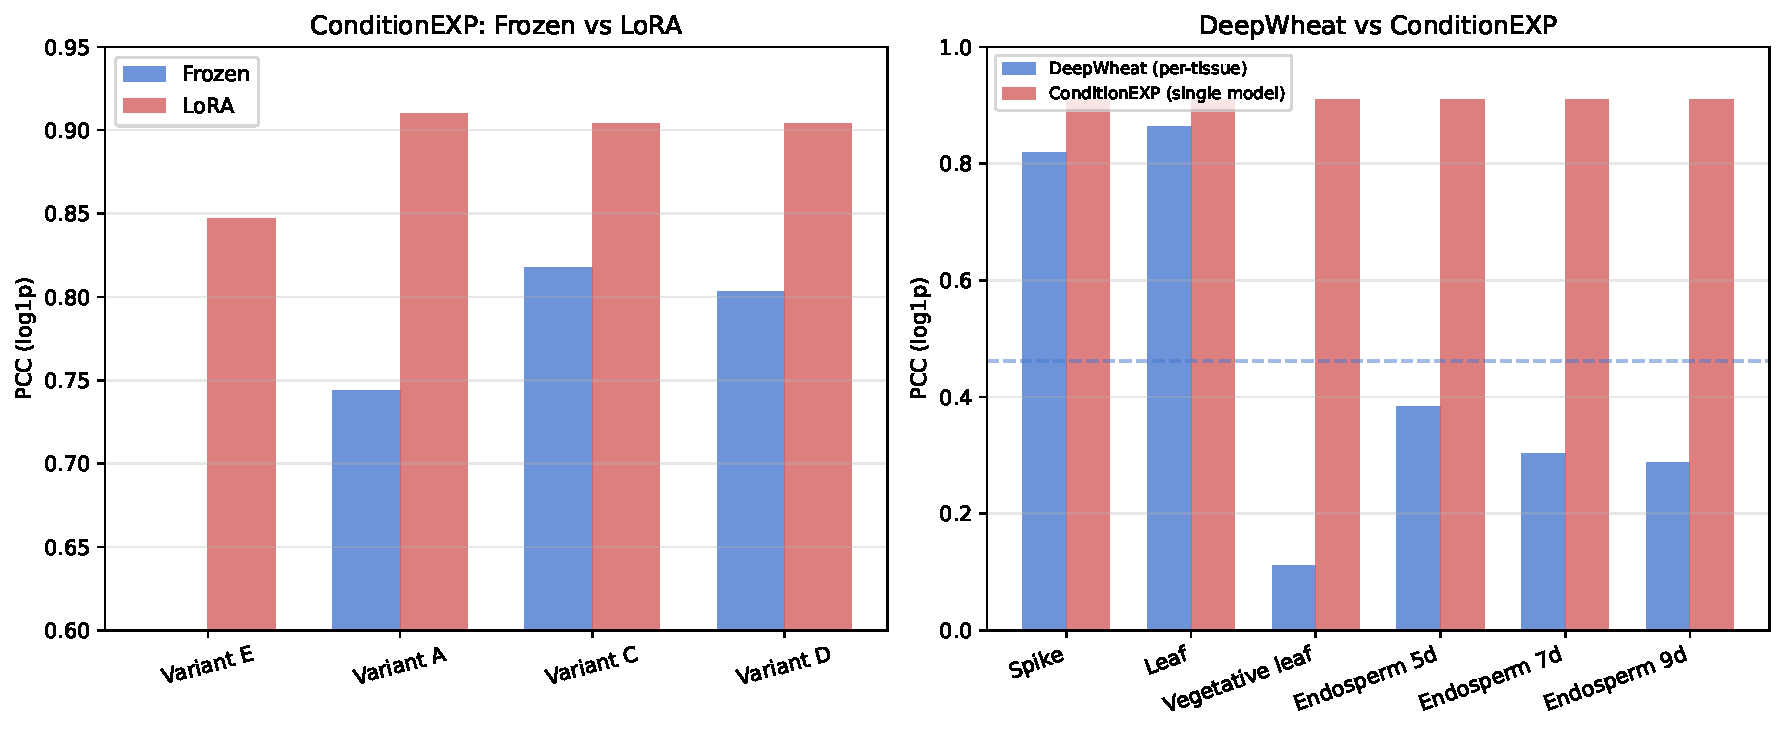
\includegraphics[width=\columnwidth]{figures/analysis2_performance_comparison.pdf}}
\caption{Performance comparison. \textbf{Left:} Frozen vs.\ LoRA-adapted embeddings across head variants. \textbf{Right:} \mytool (Variant A) vs.\ DeepWheat per-tissue performance (PCC on log-scale expression).}\label{fig:overview}
\end{figure}
